%!TEX root = thesis.tex

\renewcommand{\TheTitle}{Effect of Fuel Bed Composition on Flaming Ignition Probability}
\renewcommand{\TheAuthors}{Derek Bean, David L. Blunck}

\renewcommand{\TheAddress}{
\textbf{Status: In Preparation}
}

\PaperHeader{\TheTitle}{\TheAuthors}{\TheAddress}

\chapter{\TheTitle}
\label{part:manuscript3}

\section{Abstract}
\label{sec:abtract3}
    The increasing severity of wildfires and the expansion of the wildland urban interface have placed a greater number of homes at risk for being destroyed by wildfires. Ignition of fuel beds on or near homes by embers is a significant source of fire spread and structure loss. Fire prevention and suppression efforts lack an expedient method for estimating the likelihood of ignition for the wide variety of materials around homes. 
        
\section{Introduction}\addvspace{10pt}
\label{sec:introduction3}
    Structure losses due to wildfires have increased markedly in recent years, with over 60\% of homes lost in the last 15 years occurring since 2017~\cite{Barrett2020}. One mechanism that leads to home loss during wildfires is ignition of flammable materials around a home (e.g., pine needles accumulated on a roof) by an ember~\cite{Syphard2019, Suzuki2020, Koo2010a}. The combustion of the flammable materials then ignite the structure itself, resulting the loss of the structure. When seeking to understand the processes that occur leading up to the ignition of a structure by firebrands three processes must be considered: (1) the generation of embers in the fire itself, (2) the transport of the embers to the fuel bed, and (3) the ignition of a fuel bed after the ember lands. This work focuses on event (3), specifically the processes of heat transfer and subsequent ignition that occur after an ember lands on a fuel bed. 
    
    The phenomena that occur after an ember lands can be further broken down into three categories. First the properties of the ember that lands, second the heat transfer between the ember, fuel bed, and the surroundings, and third how the fuel bed responds to the heat transfer from the ember. The response of the fuel bed to the heat transfer from the the ember is influenced by the morphology and chemical composition of the particles in the fuel bed. Fuel bed materials present in wildfires vary significantly in both morphology and chemical composition and knowledge of the effects of each on ignition are qualitative, at best. A previous study evaluated the effects of particle morphology~\cite{Bean2021} and this work seeks to identify how differences in the chemical composition of a fuel bed under attack by firebrands influence the probability of flaming ignition. 
    
    Fuel beds at risk for ignition by embers vary significantly in chemical composition which may result in differences in thermal properties and the chemical species produces during pyrolysis. Works considering ignition of fuel beds with varying concentrations of constituents have found significant variation in ignition characteristics. Cellulose fuel beds have been observed to have a lower ignition threshold when compared to grass and pine needles when put in contact by hot metal particles~\cite{Urban2018}. Interestingly, cellulose undergoes pyrolysis at either higher temperatures or later in the heating process than both lignin and hemicellulose~\cite{Yang2007a, Shotorban2018}. This suggests that the lower ignition temperature of cellulose is not due to pyrolysis occurring at lower temperatures, but to the flammability of pyrolyzates produced. 
    
    One method to evaluate the effects of chemical composition on the flammability of pyrolyzates produced, and thus ignition propensity, is through modeling of the pyrolysis process. Efforts to characterize the pyrolysis of biomass have continually improved the understanding of the chemical processes that occur in both the solid and gas phase of pyrolysis products. Recently, more inclusive pyrolysis models have been developed that improve on the initial single step Arrhenius reactions~\cite{DIBLASI199371} and more closely approximate the reactions occurring during combustion of biomass~\cite{Ranzi2008, Debiagi2015, Dhahak2019} based on the initial chemical composition of the fuels. With the development of models that are applicable to a wide range of chemical compositions and environmental factors the possibility of modelling pyrolysis and ignition of fuel beds is possible. Coupling these models with databases, such as the Bioenergy Feedstock Library~\cite{feedstock} (which contains the chemical composition information for a wide variety of materials that may be vulnerable to ember attack during a wildfire), predictions of ignition potential may be possible without data from ignition experiments. While currently available tools, like combustion models and composition databases, may be useful individually for understanding fuel bed ignition and pyrolysis, a framework linking the individual resources and knowledge to provide a general model of fuel bed ignition is lacking. Unfortunately, the current level of knowledge on the ignition threshold of materials of variable composition does not facilitate such a framework.
   
    The objective of this work is to identify how changes in chemical composition of fuel bed materials effect the probability of flaming ignition. It is anticipated that knowledge gained from this study may be used improve the understanding of fuel bed ignition for different fuels and help build a framework for estimating ignition probabilities of different fuels without the need for extensive laboratory testing.
    
    
\section{Background}
\label{sec:background3}
    Studies considering ignition have primarily focused on the influence of heat transfer and fuel bed conditions when identifying ignition parameters and the observed sensitivities to fuel bed properties are attributed to both heat transfer and chemistry related processes. The probability of ignition generally increases as the energy content of an ember increases~\cite{Hadden2011}. However, further research has indicated that energy content alone is not a sufficient indicator of ignition as a minimum ember temperature (a driver of heat flux rates) is also necessary~\cite{Zak2014}. Additionally, heat loss from embers to the surroundings has a significant effect on ignition~\cite{Fernandez-Pello2015}. While the aforementioned efforts have focused primarily on the impact of ember properties on ignition, efforts focused on the properties of the fuel bed have shown sensitivities to fuel bed material type and particle size~\cite{Urban2018}. Additionally, for fuel beds of constant particle size, an increase in the packing density of the fuel bed resulted in a decrease in the critical heat flux needed for ignition~\cite{Mindykowski2011, Hernandez2018, Rivera2020}. The observed sensitivities to fuel bed properties are likely caused by both heat transfer and chemistry related processes. Changes in the particle size of a fixed material may impact the contact area (e.g., a ball resting on fine sawdust compared to a pile of pine needles) between the ember and fuel bed; potentially reducing the amount of heat transferred through conduction as the contact area decreases. Additionally, when considering a fixed particle size fuel bed, changes in chemical composition may change the heat transfer and heating rate of the materials due to changes in the thermal conductivity of the material affecting the ignition properties of the material. For these reasons, knowledge of the effects of chemical composition on ignition, as it relates to thermal and chemical processes, must be addressed to accurately represent ignition properties for the wide range of materials found in fires resulting in home loss.

\section{Methods}
\label{sec:methods3}
    The 50\% probability of flaming ignition with respect to the surface temperature of a resistance heater was determined for five different materials in quiescent conditions and at a wind speed of 5.8\si{\meter\per\second}. The fuel bed materials used were Douglas-fir wood, Douglas-fir bark, pine wood, pine bark, wheat straw, and oak wood. These materials were chosen to represent a range of chemical compositions, and are materials that may be subject to ember attack in a wildland urban interface fire. Table \ref{tab:composition} shows the estimated chemical composition of the materials based on the Bioenergy Feedstock Library~\cite{feedstock}. To create fuel beds of consistent particle size,  materials were granulated and then sorted such that the particles fit through a screen with openings of 2.1\si{\milli\meter} but not through openings of 0.85\si{\milli\meter}. Once sorted, the materials were oven dried at 103\si{\celsius}.
    \begin{table*}[hpbt]
        \caption{Proportion of cellulose, hemicellulose, and lignin of the materials tested estimated from the Bioenergy Feedstock Library~\cite{feedstock}}
        \centering
        \begin{tabular}{crrrr}
            % \rowcolor{gray!50}
            Material & Cellulose (\%) & Hemicellulose (\%) & Lignin (\%) & Other (\%) \\
            \hline
            Oak Wood         & 45 & 22 & 24 & 9\\
            Douglas-fir Wood & 44 & 22 & 28 & 6\\
            Wheat Straw      & 44 & 27 & 19 & 10\\
            Pine Wood        & 40 & 30 & 20 & 10\\
            Pine Bark        & 39 & 17 & 37 & 7\\
            Douglas-Fir Bark & 26 & 11 & 59 & 4 
        \end{tabular}
        \label{tab:composition}
    \end{table*}
        \begin{table*}[hpbt]
        \caption{Average bulk density of materials for each material and wind speed.}
        \centering
        \begin{tabular}{crr}
            % \rowcolor{gray!50}
            Material & U\textsubscript{bulk} = 0.1\si{\meter\per\second} (\si{\kilogram\per\cubic\meter})& U\textsubscript{bulk} = 5.8\si{\meter\per\second} (\si{\kilogram\per\cubic\meter})\\
            \hline
            Oak Wood         & 344 & 428 \\
            Douglas-fir Wood & 99  & 74 \\
            Wheat Straw      & 85  & 85 \\
            Pine Wood        & 114 & 115 \\
            Pine Bark        & 215 & 172 \\
            Douglas-Fir Bark & 131 & 146  
        \end{tabular}
        \label{tab:composition}
    \end{table*}
    Two experimental apparatus were used to conduct ignition experiments. The experimental apparatus used for the tests in quiescent conditions is shown in Figure~\ref{fig:speciesApparatus}. The quiescent apparatus used a lever arm to hold the cartridge heater in a fixed position the duration of the test. The heater was inserted into the fuel bed approximately half of the heater diameter (3\si{\milli\meter}). Tests conducted with a wind speed of \si{\meter\per\second} were performed using the apparatus shown in Figure~\ref{fig:speciesWindTunnel}. This apparatus was operated inside of a wind tunnel where the heater was lowered using an automated lowering device that maintained a constant pressure equivalent to that of a 10\si{\gram} ember landing on the fuel bed. The pressure was monitored and adjusted using a PID control system with force measured by a load cell. For all tests the cartridge heater (firebrand surrogate) used was a 50\si{\milli\meter} long 6.35\si{\milli\meter} diameter cartridge heater.
        \begin{figure}[htpb]
        \centering
        \resizebox{\figureWidthSet}{!}{%
        \begin{tikzpicture}
            \filldraw [draw=black!60, pattern=north west lines, pattern color= brown] (0, 0) rectangle (140mm, 70mm) node[pos=0.5, fill=white] {\Huge Fuel Bed}; 
            \filldraw[] (0mm, -2mm) rectangle (140mm,0mm) node[rotate=-90, pos=0.5] {};
            \filldraw[] (-2mm, -2mm) rectangle (0mm,70mm) node[rotate=-90, pos=0.5] {};
            \filldraw[] (140mm, 70mm) rectangle (142mm,-2mm) node[rotate=-90, pos=0.5] {};
            \filldraw [fill=red, draw=black] (45mm, 67mm) rectangle (95mm, 73mm) {}; 
            \filldraw [draw=black, fill=black!50] (55mm, 65mm) rectangle (58mm, 85mm) {};
            \filldraw [draw=black, fill=black!50] (66mm, 85mm) rectangle (48mm, 185mm) {};
            \filldraw [draw=black, fill=black!50] (-85mm, 220mm) rectangle (-67mm, -2mm) {};
            \filldraw [draw=black, fill=black!50, rotate around={-15:(57mm, 100mm)}] (66mm, 95mm) rectangle (-100mm, 105mm) {};
            \filldraw [draw=black, fill=black!50, rotate around={-15:(57mm, 170mm)}] (66mm, 165mm) rectangle (-100mm, 175mm) {};
            \filldraw [draw=black, fill=black!50] (-90mm, -2mm) rectangle (150mm, -4mm) {};
            \filldraw (57mm, 170mm) circle (2mm);
            \filldraw (57mm, 100mm) circle (2mm);
            \filldraw (-76mm, 205mm) circle (2mm);
            \filldraw (-76mm, 135mm) circle (2mm);
            \filldraw [rotate around={15:(140mm, 85mm)}] (140mm, 85mm) rectangle (145mm, 90mm) node[above right] {\Huge Photodiode};
            \draw [<-, line width=1mm] (75mm, 75mm) -- (125mm, 120mm) node[right] {\Huge Heater};
            \draw [dashed] (140mm, 87.5mm) -- (100mm, 72mm);
            \draw [dashed] (140mm, 87.5mm) -- (80mm, 74mm);
        \end{tikzpicture}
        }
        \caption{Experimental apparatus for the ignition tests. The lever arm used to lower the apparatus into the fuel bed, the fuel bed size relative to the heater, and the location of the photodiode are illustrated.}
        \label{fig:speciesApparatus}
    \end{figure}
    The temperature of the heater was recorded with a type-K thermocouple for the duration of each test. The temperature of the heater for ranged from 250\si{\celsius} to 750\si{\celsius} and was controlled using PID control logic implemented in LabVIEW. The PID controller kept the heater temperature within 6\% of the setpoint for the duration of the tests. The temperature setpoints of the resistance heater were determined using the three-phase optimal design procedure to efficiently determine the desired ignition probability for the number of tests conducted~\cite{Wu2014}. For tests where flaming ignition did not occur data was recorded for 3000\si{\second} or until the reaction front of the smoldering material reached the edge of the test container. The fixed position of the cartridge heater and the use of the cartridge heater was implemented to maintain consistency between tests of the same material and between test series of different materials. The use of the cartridge heater and the fixed position is not necessarily representative of a burning ember landing on the fuel bed but the consistency of surface temperatures, ability to record temperature, and consistent contact with the fuel bed are essential for comparing results across test series and materials. For the quiescent tests flaming ignition was detected with the use of a BPX 65 photodiode sampled at 1 kHz. If the intensity detected rose above a set threshold flaming ignition was said to occur. For the wind tunnel tests flaming ignition was determined from the rising temperature of the cartridge heater in the presence of flame. Visual detection of flames was also used in cohort with the photodiode measurements. The 50\% probability of ignition was determined from a logistic regression on the outcomes of 25 ignition tests conducted for each of the materials for which flaming ignition was observed. The scikit-learn python package~\cite{scikit-learn} was used to perform the logistic regressions used to predict ignition probabilities.
    \begin{figure}[hbpt]
            \centering
            \resizebox{0.5\columnwidth}{!}{%
                \begin{tikzpicture}
                    \filldraw[pattern=north west lines, pattern color=brown, thick] (2.84, 0)  rectangle (4.34, -.75) node[pos=0.5,rectangle,fill=white] {\scriptsize Fuel Bed};
                    \fill [draw=white,  inner color=red, outer color=white ] (3.59, 0.01) circle (0.15);
                    \filldraw[draw=black,fill=white, thick] (0, 0)      rectangle (6, 3);
                    \fill[fill=black!50] (3.58, 0) rectangle (3.61, 1.52);
                    \fill[fill=black] (3.55, 1.52) rectangle (4.23, 1.57);
                    \filldraw[draw=black, fill=black!50] (4.09, 1.57) rectangle (4.22, 3);
                    \fill[draw=red, fill=red] (3.59, 0.01) circle (0.0635);
                    \draw [<-] (3.5, 0.1) -- (3, 0.5) node[left] {\scriptsize Heater};
                    \draw [<-] (3.5, 1.55) -- (3, 1.55) node[left] {\scriptsize Load Cell};
                    \draw [<-] (3.75, 2.5) -- (3, 2.5) node[left] {\scriptsize Lowering Arm};
                    \draw[->]         (0.1, 0.6) -- (0.75, 0.6);
                    \draw[->]         (0.1, 1.2) -- (0.75, 1.2);
                    \node[right] at (-0.75, 1.5) {\scriptsize Inlet};
                    \draw[->]         (0.1, 1.8) -- (0.75, 1.8);
                    \draw[->]         (0.1, 2.4) -- (0.75, 2.4);
                    \draw[draw=black, dashed] (3.336, 0) rectangle (4.54, 0.34);
                    \draw[->]         (4.3, 1) -- (4.0, 0.34);
                    \node[right, align=left] at (4.3, 1) {\scriptsize Computational\\ \scriptsize Domain};
                \end{tikzpicture}
                }
            \caption{Diagram of the experimental wind tunnel apparatus. Air flows through the wind tunnel from left to right. The dashed region represents the domain subset used for computational efforts.}
            \label{fig:speciesWindTunnel}
        \end{figure}

    
\section{Results and Discussion}
    \label{sec:results3}
    The flaming or non-flaming ignition outcome of each test and the logistic regression results for Douglas-fir wood, oak wood, and pine wood are shown in Figure~\ref{fig:logistic_plot} for the quiescent tests. The circular markers represent the outcome of each test, either flaming or no ignition. The logistic regression for each material is shown as a solid line with the shaded regions representing the 95\% confidence interval for each regression. Douglas-fir bark, pine bark, and wheat straw are not shown in Figure~\ref{fig:logistic_plot} because flaming ignition was not observed for five tests at the maximum heater temperature of 750\si{\celsius}. The heater temperature estimated to produce 50\% ignition probability from the logistic regressions for each material is shown in Figure~\ref{tab:composition50temp}. Anecdotally, self sustained smoldering was observed for all five materials at temperatures lower than the flaming ignition temperature. The heater temperature corresponding the onset of smoldering ignition was not measured in this study. 
        \begin{figure}[htpb]
            \centering
            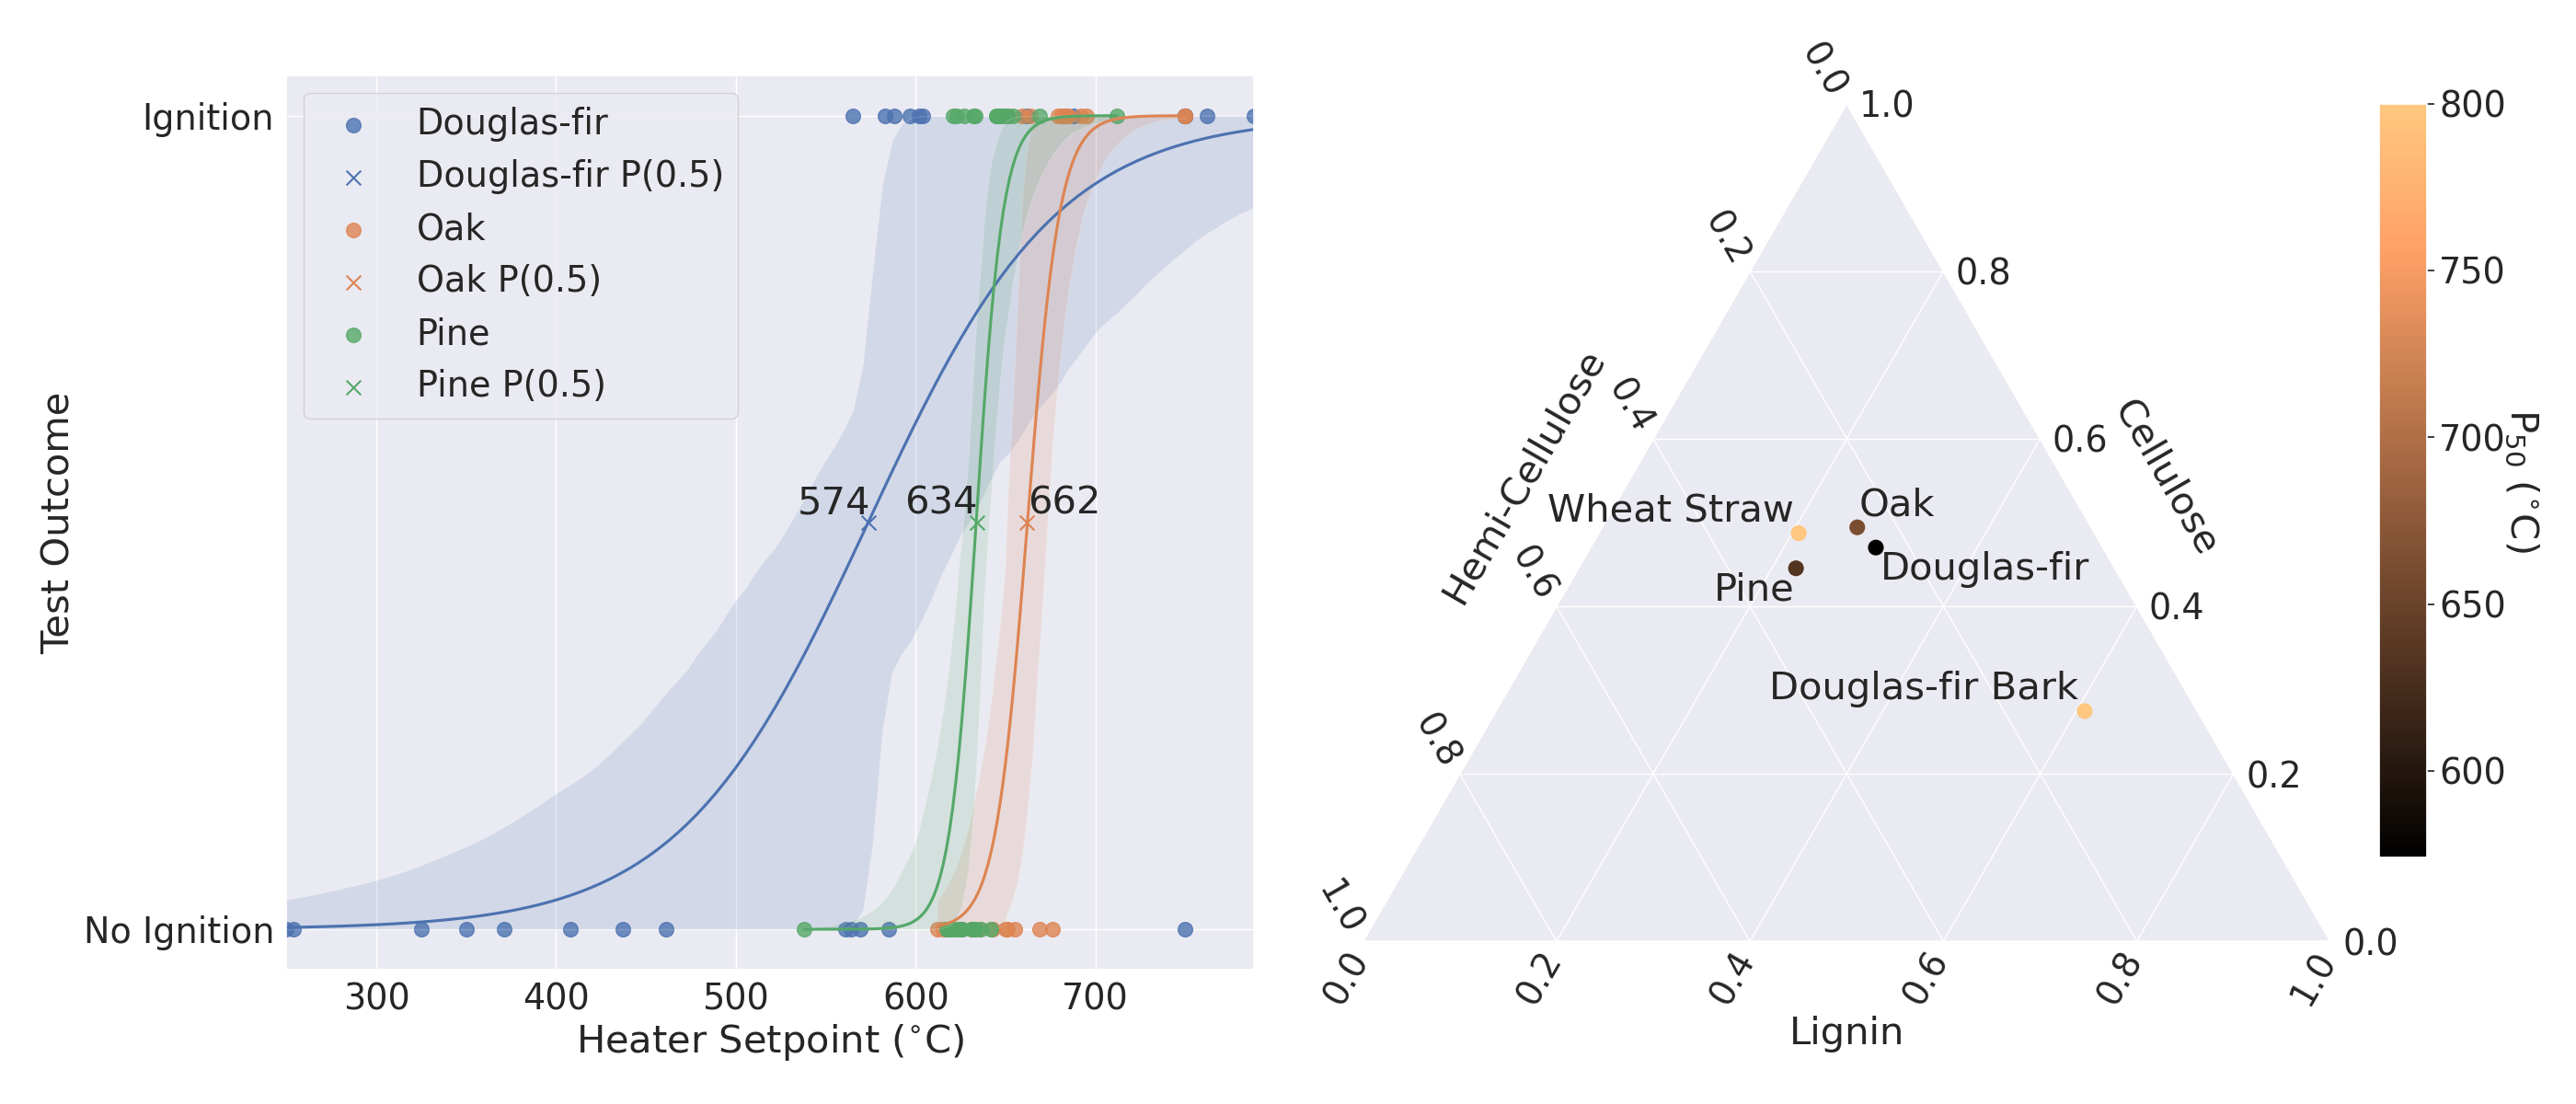
\includegraphics[width=\figureWidthSet, trim={0 0 37cm 0}, clip]{conference_results_binary.png}
            \caption{Test results for materials where flaming ignition was observed. The circular markers denote individual tests. The solid lines represent the logistic regression and the shaded zones the 95\% confidence interval with the 50\% probability of ignition labelled}
            \label{fig:logistic_plot}
        \end{figure}
    Two aspects of the ignition results are of note from the quiescent cases. As anticipated, the differences in estimated heater temperature to produce 50\% ignition probability suggest that significant differences in ignition occur across a range of materials in the same apparatus and experimental conditions. Second, the transition between no ignition and flaming ignition may become less defined (i.e., the 95\% confidence interval of the regression spans a much larger temperature range) as the ignition temperature decreases. This is significant because it may cause more difficulty in predicting the ignition of materials that ignite at lower temperatures. Lower confidence in predicting ignition for easily ignitable materials would be detrimental to the usefulness of a model or predictive tool that may be implemented from this testing methodology. It is, however, unclear if the ignition to no ignition transition in other materials of similarly low ignition temperature will behave similarly to that of Douglas-fir. Characterization of additional materials is needed to elucidate these trends.
    
    Figure~\ref{fig:composition_plot} shows the averaged cellulose, hemicellulose, and lignin concentrations for each material according to the samples recorded in the Bioenergy Feedstock Library as shown in Table~\ref{tab:composition}. The marker colors for each material correspond to the calculated 50\% ignition probability for the quiescent tests except for the wheat straw and Douglas-fir bark which are denoted as 800\si{\celsius} to indicate that the 50\% ignition probability was higher than the temperatures tested.  Note that due to scaling inherent to a ternary projection the proportion of the fuels characterized as other causes a shift in the data. For example, the wheat straw and Douglas-fir are estimated to have the same cellulose content but do not lie on the same iso-line of 44\% cellulose. Nonetheless, the relative proportions of each constituent are retained and comparisons may still be made. 
        \begin{figure}[htpb]
            \centering
            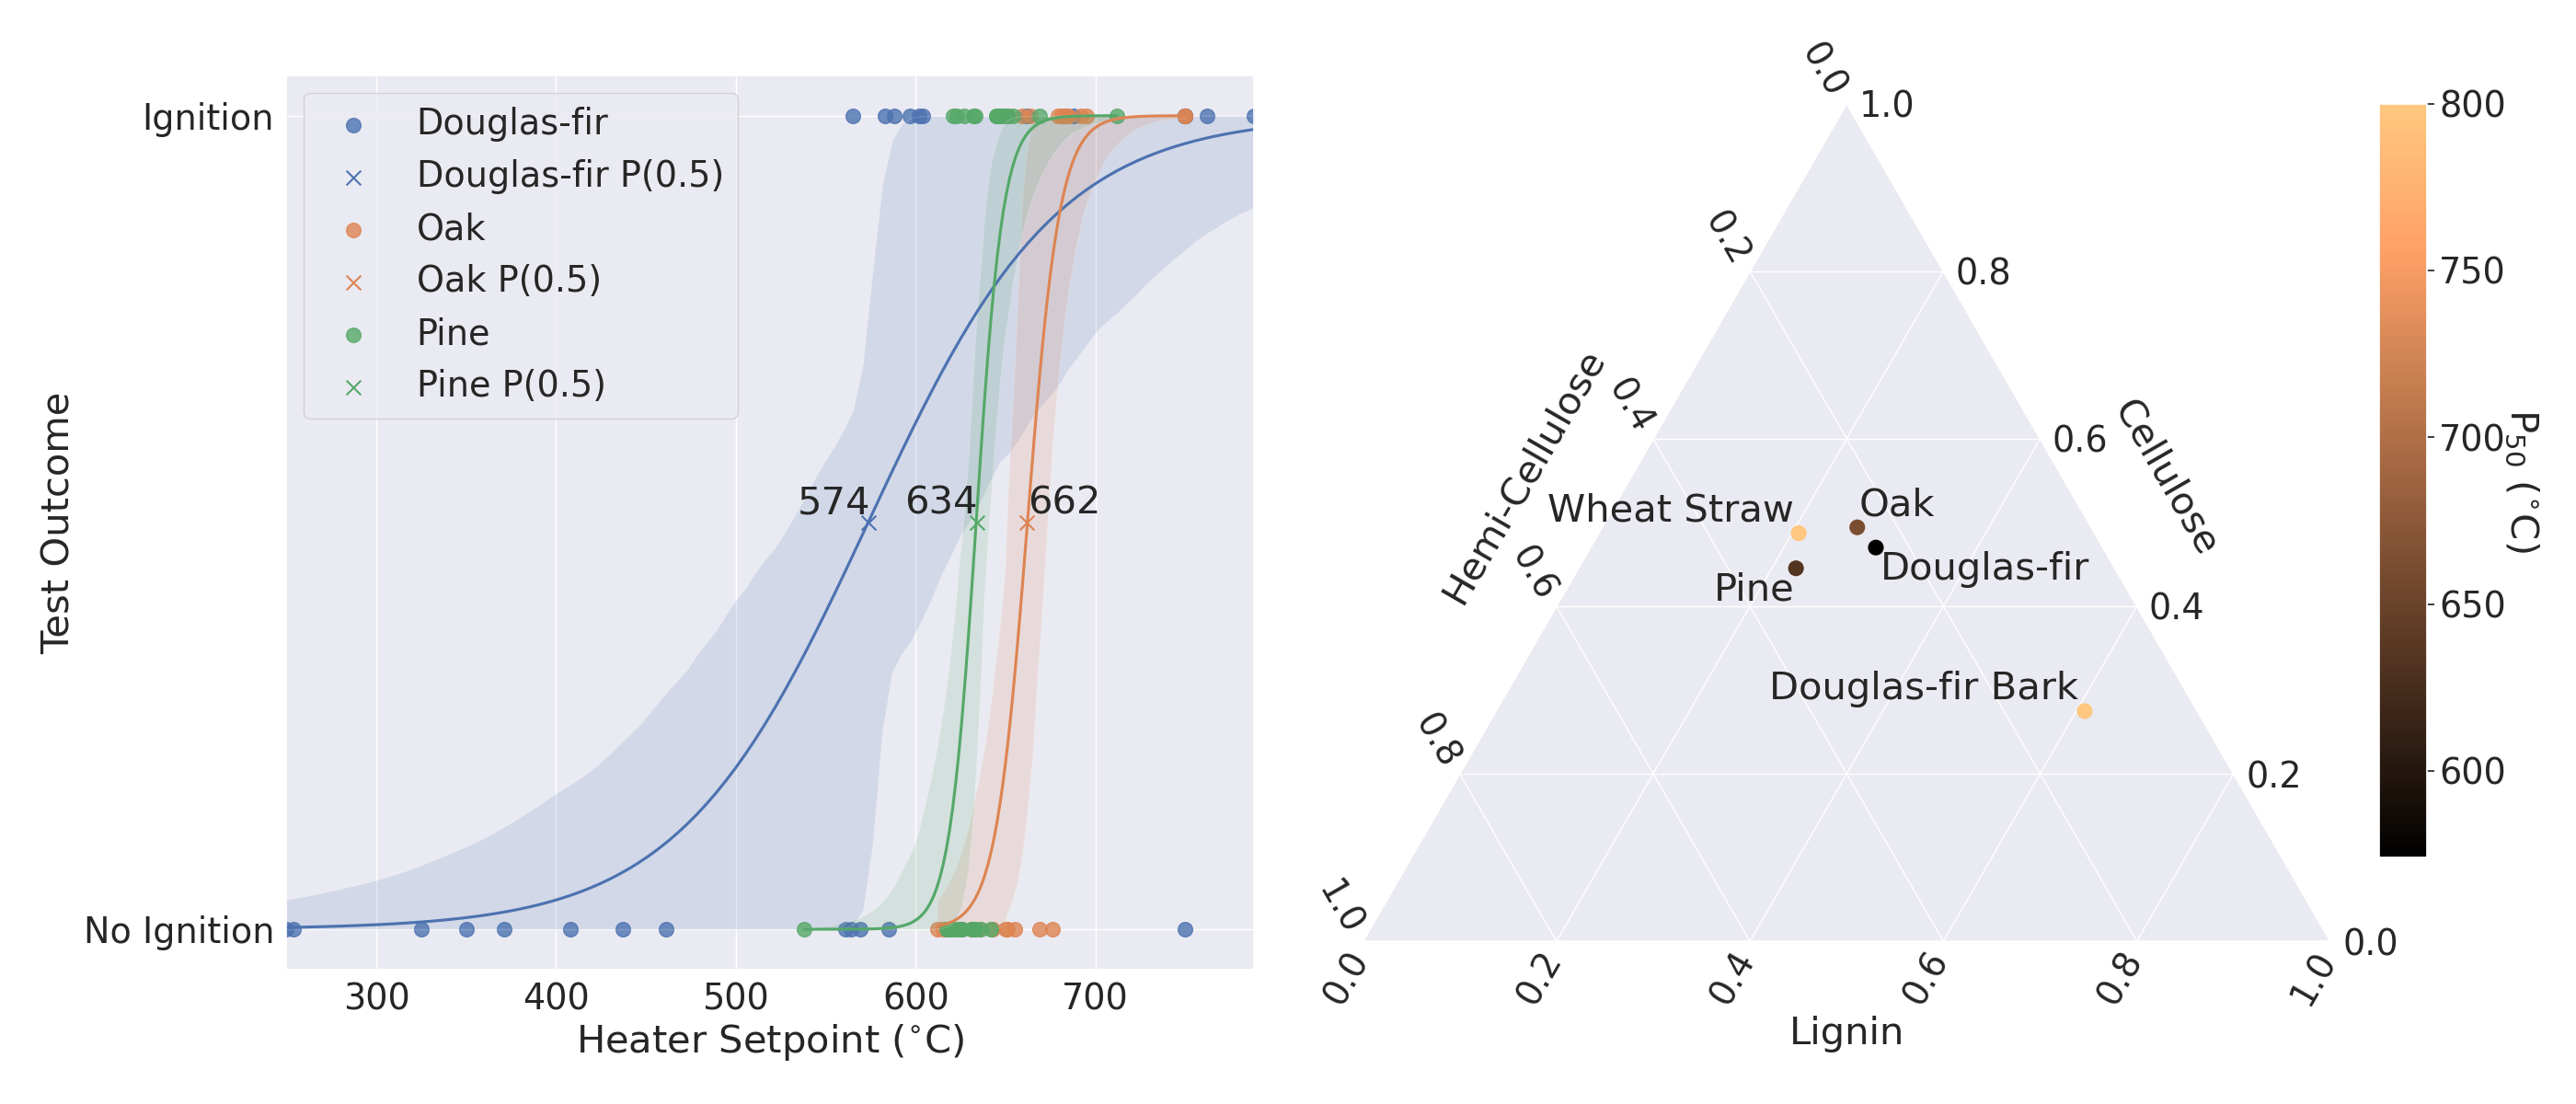
\includegraphics[width=\figureWidthSet, trim={35cm 0 0 0}, clip]{conference_results_binary.png}
            \caption{Estimated chemical composition of each material tested with the marker color representing the estimated 50\% ignition probability. Note that the materials where flaming ignition did not occur are represented as 800\si{\celsius} to show that the temperature of ignition was not achieved.}
            \label{fig:composition_plot}
        \end{figure}

    Perhaps unsurprisingly, Douglas-fir bark and pine bark, with the highest lignin content, were not observed to ignite for the conditions tested. This suggests that materials with high lignin contents may be the least likely to ignite when exposed to embers and thus are the safest with respect to flaming ignition risk around homes. This does not, however, account for the potential for smoldering ignition and a subsequent smoldering to flaming transition that may occur. Thermogravametric analysis experiments have shown that while lignin begins to decompose at the lowest temperature of the three primary components, it decomposes at the slowest rate and at a much wider range of temperatures~\cite{Yang2007a}. It was also observed that the peak gas production of \ce{CO}, \ce{CO2}, and \ce{CH4} occurs at a higher temperatures than hemicellulose and cellulose. In contrast to Douglas-fir bark, wheat straw had the lowest estimated lignin concentration but was also not observed to ignite. When comparing wheat straw to Douglas-fir wood the higher lignin concentration suggests that Douglas-fir wood is likely to have a higher ignition temperature than wheat straw. This discrepancy is attributed to two material attributes. First, the pyrolysis process is complex and there is not a clear linear relationship between the composition of the fuel and flaming ignition. It appears that materials of different compositions are capable of producing gaseous products of near equal ignitability but the proportion of each constituent for which ignition to occurs most readily is unclear. Second, the thermal conductivity of the materials likely varies significantly which impacts the temperature gradients and mass of the material above the pyrolysis temperature, further obfuscating the effect of composition on ignition. 
    
    The 50\% ignition probability results for the 5.8\si{\meter\per\second} wind speed tests are shown in Table~\ref{tab:composition50temp} along with the results for the 0.1\si{\meter\per\second} tests. From these results there are three observations of note. First, the increase of wind lowered the threshold for ignition probability for the Douglas-fir wood and Pine wood by approximately 30\%. Second, in contrast to the Douglas-fir and Pine wood results, an increase in wind resulted in a decrease in a higher threshold for ignition.  Third, the materials that were not observed to ignite in the quiescent tests were also not observed to ignite in the presence of wind. While the trends for douglas-fir wood and pine wood match those presented in Chapter~\ref{part:manuscript2} and trends reported in other studies of pine needle ignition~\cite{Wang2017} and eucalyptus bark~\cite{Ellis2011, Ellis2015}. The decreasing ignition probability of the oak wood contradicts those observed in the aforementioned studies and this study but is not unprecedented. Ignition studies of various litter layers types ignited by various single firebrands observed a sensitivity to ember location where embers that landed on top of a fuel bed in windy conditions were less likely to cause ignition than those embedded where ignition was enhanced~\cite{Plucinski2008}. This trend was attributed to increased heat loss due to wind. In this study, however, the location of the cartridge heater was consistent across all materials, the energy is not a function of the wind speed, and the flow field around the embers is consistent.  
    \begin{table*}[hpbt]
        \caption{Heater temperature required for 50\% probability of ignition for the materials and conditions tested.}
        \centering
        \begin{tabular}{crrr}
            % \rowcolor{gray!50}
            Material & 0.1 \si{\meter\per\second}(\si{\celsius}) & 5.8 \si{\meter\per\second} (\si{\celsius}) & $\Delta$T (\si{\celsius})\\
            \hline
            Douglas-fir Wood & 574  & 391 & -185 \\
            Pine Wood        & 634  & 430 & -204\\
            Oak Wood         & 663  & \textgreater750 & 87\\
            Wheat Straw      & \textgreater750 & \textgreater750 & -\\
            Pine Bark        & \textgreater750 & \textgreater750 & -\\
            Douglas-Fir Bark & \textgreater750 & \textgreater750 & -
        \end{tabular}
        \label{tab:composition50temp}
    \end{table*}
    
    Comparing the ignition trends of oak wood to the non ignition of pine bark and douglas-fir bark it would seem that a potential cause of decreased ignition is correlated to the material properties. Density particle size chemistry
    
    
    
    In summary, characterizing the flaming ignition propensity of fuels with respect to chemical composition alone will likely not yield satisfactory results. The inclusion of other material properties, such as thermal conductivity, however, may add enough additional knowledge for comprehensive predictions of ignition to be made. Further investigation of the differences in chemical and thermal properties of the materials is necessary to unravel the interactions between thermal and chemical processes and the resulting impact on flaming ignition before knowledge sufficient for a predictive tool that may be used for fire prevention and management may be created
    \cite{MacLean1941}.
    

    
   